\documentclass[a4paper,12pt]{article}

\usepackage{url, hyperref, graphicx}

\begin{document}

\title{Project 2}
\author{Chip Bell}
\date{April 24, 2015}
\maketitle

\section{Problem Description}
The Washington Metropolitan Area Transit Authority's Metrorail system in many respects is a driving factor in the
expansion of the city. With Washington's fixed size, reliable and cost-efficient transportation for metro area
residents is crucial for maintaining the city's economy. However, this is a difficult task in that there are many
variables involved, such as human error, mechanical failure, and even acts of nature.

Therefore for this project, I will be simulating the metrorail system using data collected from the WMATA API
\cite{wmataapi}, which provides realtime estimates of train arrival. Furthermore, I will simulate the impact that track
closures have on train throughput.

\section{Previous Work}
Many large cities have rapid transit systems, so considerable research time has been invested on building reliable
subways. Commercial software such as OpenTrack \cite{opentrack} have been developed, and even video games such as Train
Simulator \cite{trainsimulator} and Open Rails \cite{openrails}. Algorithms for handling single, double and triple tracks exist,
such as a basic
algorithm for sharing tracks between trains presented by Fiorini and Botter \cite{fioroni}. Dessouky and Leachman
\cite{dessouky_leachman_95} provide an event-driven algorithm for single and double track rail networks, incorporating
acceleration. Lu et al \cite{quan_lu} expand the model to triple tracks while enhancing the acceleration model to
handle multiple track speed limits.

\section{Basic Architecture}
The nature of trains lends itself to a model that incorporates resource sharing. For instance, only a single train can
occupy a particular section of track at a given moment. Furthermore, if two trains are sharing a track, they cannot
be going in different directions unless they have already past each other, lest they collide. This issue is addressed
by Fioroni \cite{fioroni}.

A common occurrence in the metro system is that between two stations a particular section of track is under
maintenance, forcing trains going both directions to share a track. These basic issues result in a couple of clear
concepts that we'll incorporate in our model.

The first is a train. A \texttt{Train} encapsulates all of the information relevant to our application: which line it is
(Orange, Blue, or Silver), it's direction, and it's location within the system. Measuring the throughput of trains
in the system will be our primary statistic when running the simulation.

The other important entity to be concerned with is the track itself. In the simulation, this is modeled using a
\texttt{TrackSegment} class. A \texttt{TrackSegment} is simply a queue with the ability to be process \texttt{Train}s
one at time.

From a queueing standpoint, a \texttt{TrackSegment} is a limited
resource that only a single train can use at a single point. If a piece of track is occupied by a train, all other
trains must wait before they may proceed through the track (in an assumed FIFO order). It is for this reason that
most train systems do prefer to have a second track to prevent blocking for trains going in opposite directions.
So, in our case we can treat a section of track as a queue that can only process a single train at a time. Between
stations, there are generally two sections of track. However, track maintenance would cause a track to close, forcing
opposing tracks to share.

Because of this, we can represent the entire metro as queuing network with sections between stations as the queue. In
our case, we will only be modeling the section of track between Rosslyn and Stadium-Armory where the Orange, Blue, and
Silver share a track (See \ref{fig:metromap}). Since there are no track crossovers, we can consider these three lines
to be isolated from other lines. However, we do need to keep in mind that for two tracks, each track is devoted to a
specific direction. Only in the case of a single track is when a track will handle both directions.

I've also chosen to conceptually model pairs of tracks between stations as a \texttt{StationConnection} class. Perhaps
unsurprisingly, this is the largest and most important class in the simulation, since it manage two
\texttt{TrackSegment}s, along with the disabling/enabling of a track segment. When a track is disabled, the
\texttt{StationConnection} must begin routing trains through a single track, rather than reserving tracks for
only particular directions. This logic is important to the accuracy and realism of the simulation, since it's one of
fundamental principles behind a train track. 

Because this will be a discrete-event simulation, we will need to be mindful of the events that travel through our
application. A first example that comes to mind is the \texttt{train:arrive} event, which will be received by the
Rosslyn and Stadium-Armory stations when a train first arrives in the system. This event will need to contain the train
instance, along with the direction its heading (although that is implied by the station in our case). This way, we can
track the train as it moves through the system to calculate metrics about the system's performance.

When a train first arrives at a station, it is queued up to await a free track. If the track designated for that
direction is already available, the train simply moves on to the track and occupies it until it reaches the next
station where it exits and then queues up at the next station.

When a train is dequeued and allowed to enter a track, a \texttt{train:enter} event is thrown. When this event occurs,
the station connection marks the track as occupied so that later arriving trains do not attempt to enter the track. The
connection also schedules a new event: \texttt{train:exit}

\texttt{train:exit} is triggered when a train exits a connection, which informs a connection to free up the track and
push the next train through if there is one. As mentioned before, this event is actually scheduled when a train enters
a track between stations. Each connection has knowledge of the time between it's associated stations, and uses that
time to schedule the \texttt{train:exit} in relation to \texttt{train:enter} for a particular train. Lastly, when a
train exits a particular connection, a \texttt{train:arrive} event is scheduled immediately for the next connection in
the metro system.

\begin{figure}
\begin{center}
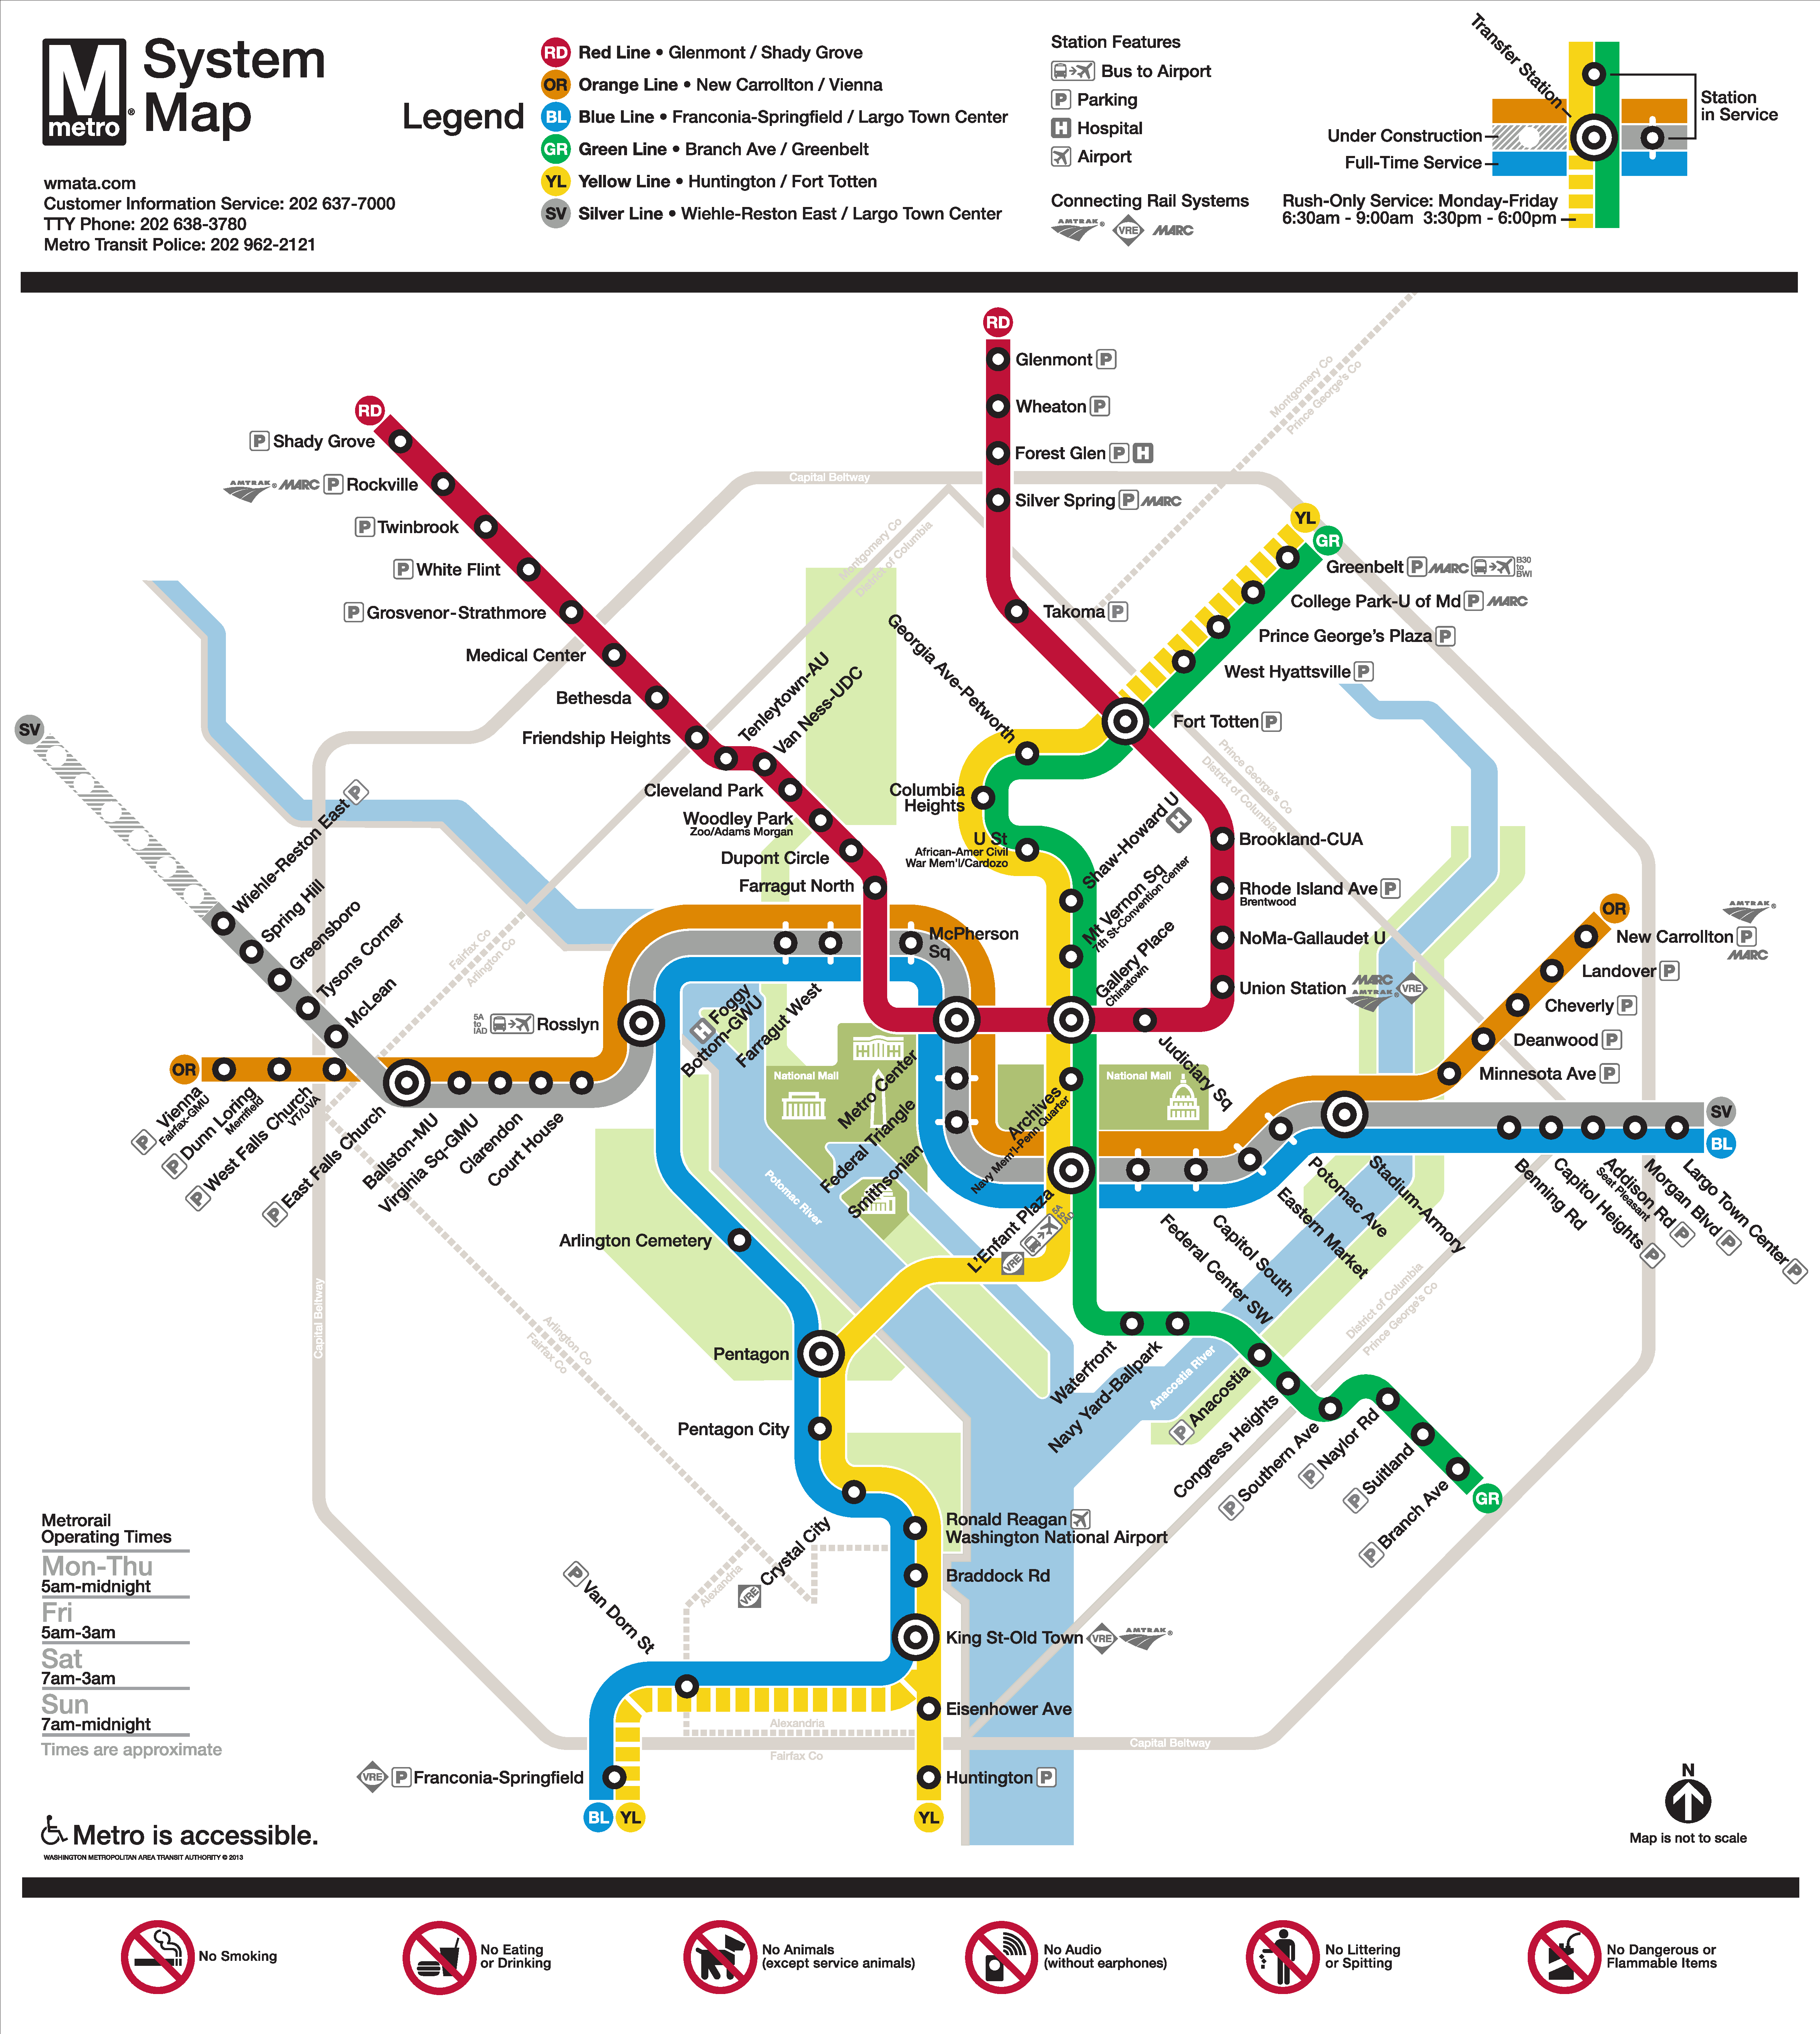
\includegraphics[width=5in]{../images/metro_map.pdf}
\caption{\small \sl WMATA Metrorail Map \label{fig:metromap} \cite{fioroni}}
\end{center}
\end{figure}

\section{Data Collection}

\subsection{Query Design}
Viewing this as a queueing problem, there are some ``missing pieces'' that our model did not incorporate, namely the
arrival rate of trains and the service time for a single train. Instead of attempting to calculate these based on 
numerical models of motion, we can instead use the WMATA API \cite{wmataapi} to calculate this.

The API provides data by station with an estimate at each station of the wait time until the next train. For instance,
the API for a station on the blue line might list a train to Franconia-Springfield (westbound) in 1 minute. If there
also happens to be an Orange that passes through that station, you may also see an estimate for the next Orange (if it
is close enough).

Given this information, we can calculate how often a train runs simply by marking the timestamp of the API call and
offset by the estimated time until arrival provided by the API. For instance, if we query a station at 12:00 PM, and
the API estimates a train arriving in 3 minutes, we can roughly estimate that the train will arrive at 12:03. This
gives us our arrival rate. Furthermore, we can query by train line as well to verify that trains run according to the
schedule that WMATA provides on its website \cite{metroschedule}.

To calculate service times for a particular section of track, we need an estimate of the time it takes for a train to
travel between two stations. This is clearly station dependent, since some stations are closer than others. However,
all but one of our stations are within the District of Columbia, so we expect the travel times to be small.

We can still calculate an estimated travel time between two stations through the API as well. Given two neighboring stations $A$ and $B$, if
we query $A$ for an upcoming trains of color $c$ in the direction of $B$, we will get some estimate for the arrival. We
can query $B$ for the same color train in the same direction to obtain a estimate of the arrival time at $B$.
Subtracting these two numbers provides an estimate of the travel time between stations. This makes an assumption that
there is no train of the same color in the middle that may skew the estimate. However, we can minimize the chance of
this happening if we restrict our queries on $A$ to trains that are only a minute away. Given that the stations are so
close, we minimize the likelihood that there is a ``middle train'' that causes inaccurate estimates.

\subsection{Query Results}
A script was built to call the WMATA API for train estimates, and was setup as a cron job on server. The script
essentially downloaded the estimates of train arrivals for every station into a single timestamped JSON file (see the
JSON format \cite{json}. Cron \cite{crontab} was configured to run the script every minute for an entire week,
resulting in a directory full of timestamped JSON files. These were then imported into a Mongo \cite{mongodb} database 
to allow easier queries.

Train interarrivals were measured by line and direction. \ref{fig:eastboundblueinterarrivals} demonstrates a case where
the data appears to be normal. However, other cases such as \ref{fig:westboundsilverinterarrivals} show that this is
not necessarily true. Graphs for the remaining directions and line colors were omitted for brevity, but are included in
the submission. Due to time constraints, we'll use an empirical distribution rather than trying to fit any particular
distribution.

\begin{figure}
\begin{center}
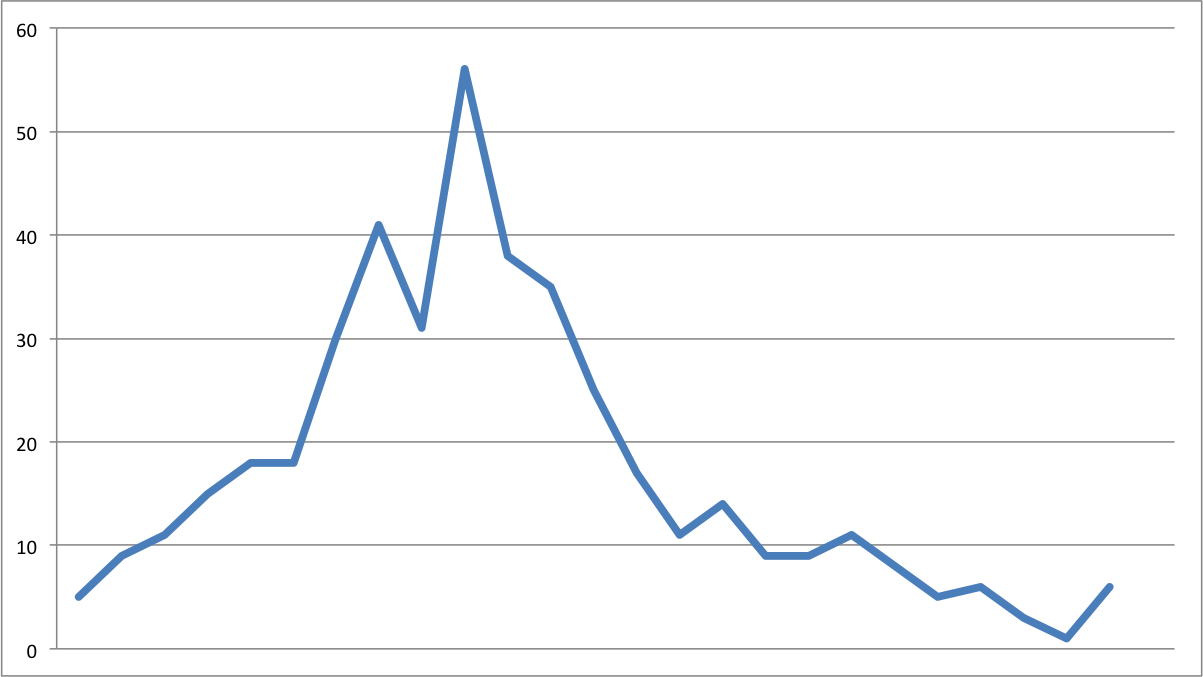
\includegraphics[width=4in]{../images/train_interarrivals/eastbound_blue_interarrivals.png}
\caption{\small \sl Eastbound Blue Line Interarrivals at Rosslyn. Ranges from 2.71 minutes to 16.78 with mean 10.91 minutes \label{fig:eastboundblueinterarrivals}}
\end{center}
\end{figure}

\begin{figure}
\begin{center}
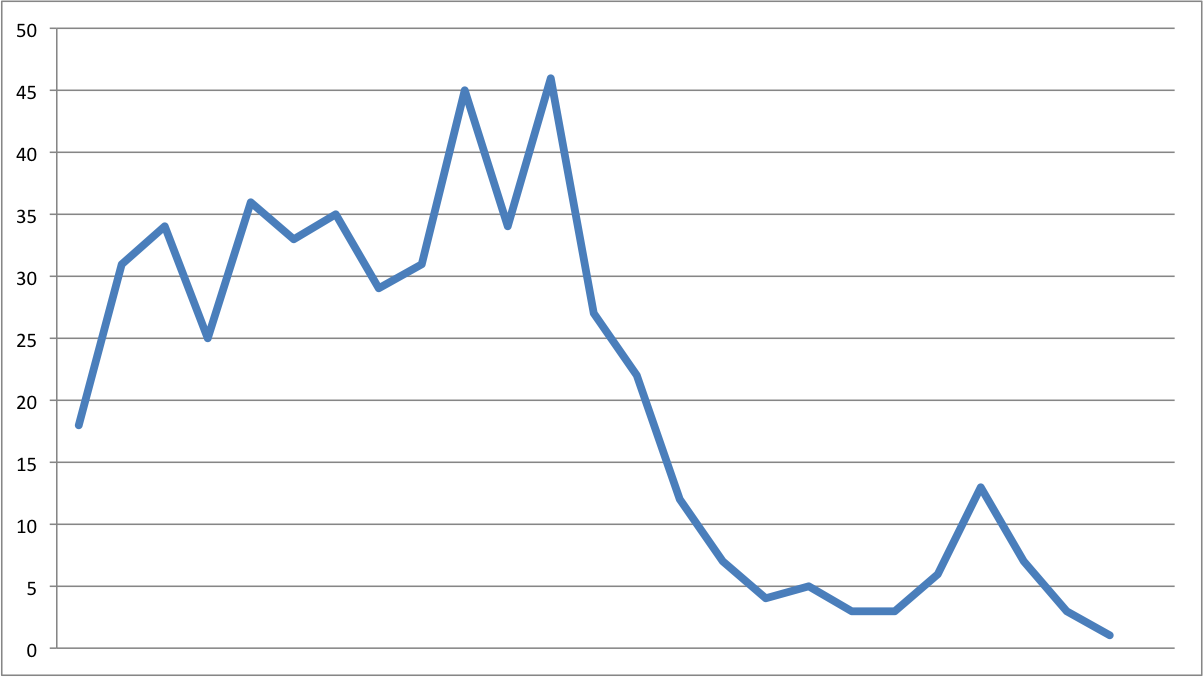
\includegraphics[width=4in]{../images/train_interarrivals/westbound_silver_interarrivals.png}
\caption{\small \sl Westbound Silver Line Interarrivals at Stadium-Armory. Ranges from 2 minutes to 24 with mean 9.25 minutes \label{fig:westboundsilverinterarrivals}}
\end{center}
\end{figure}

Time between stations results were fairly predictable, and most stations averaged around a 2 minute travel time between
stations. However, between Foggy Bottom and Rosslyn the times instead average around a minute higher. This is simply
due to the distance between the stations, which is considerably greater between those stations.

\section{Caveats and Limitations}
With any sort of simulation of a real-world system, there are simplications and assumptions that are made, and this project is of course no
different. In some cases the reduction in detail does not harm accuracy but simply makes the model designer's and
programmer's life easier. However, sometimes this is not the case and the simplifications greatly reduce the accuracy
of the model. Thus, it is the modeler's job to judiciously choose which details to omit and leave in when building the
model.

One of the simplifications that we've made is that we've excluded all other stations in the metro system except those
between Rosslyn and Stadium Armory. Other lines, the Red, Green, and Yellow lines, do not share track with any train,
nor do they cross at any point. In this respect, they are isolated (regardless of the fact that they may share
stations). So, in this case, the simplification hinders accuracy in no way whatsoever. However, ignoring Blue, Orange,
and Silver stations beyond Stadium-Armory and Rosslyn could potentially
reduce model accuracy here because train events at those stations can very easily influence the stations within D.C.
We have chosen instead to model those exterior stations as a probability distribution which is based off of empirical
data, but we still run a risk that we may have not captured an important interaction.

That being said, choosing an empirical distribution like we have has the potential to be a wise or poor choice. If the
"true distribution" of train interarrivals and between station times abides by what we have observed, then our choice
of empirical distribution was smart, and we've saved ourselves some effort. However we don't know the true
distribution, and it could be that our observations do not match that distribution at all.

For individual trains, we'll also ignore some of the micro-effects of acceleration and deceleration and assume our
between station times measurements captures that. For visualization purposes, we can simply draw trains as moving at a
constant velocity through the system, although this is clearly not the case.

\section{Technology Used}
The simulation was built using CoffeeScript \cite{coffeescript}, using Backbone \cite{backbone}, Underscore
\cite{underscore} and jQuery \cite{jQuery} to organize code some. Code was bundled via Browserify \cite{browserify},
and minified with UglifyJS \cite{uglify}. Gulp \cite{gulp} was used as a build tool and package management was done
via NPM \cite{npm}. Geo-mapping was done via Leaflet \cite{leaflet}, which provides an API for enhancing the map with
markers, text, shapes, etc.

In an effort to ensure code is working properly, the simulation was built with a testing suite. Mocha \cite{mocha} was
used as the testing framework, and Chai \cite{chai} was used for BDD-style assertions. Sinon \cite{sinon} was used to
mock function calls during tests.

\section{Current Build and Instructions}
Currently, the app is simply mapping stations and labeling them based on information provided by the API. The entirety
of data analysis is complete, and can be
viewed within the \texttt{queries} directory, along with the \texttt{utils}. A few data files are strewn about the
codebase as well. The WMATA API query code is stored within the \texttt{wmata} folder.

I have also copied some code over from the first project since it will be applicable, such as a discrete event queue.
However, the \texttt{Track} class remains to be written and is integral to the application, along with the \texttt{Train}
class. Furthermore, the actual
train scheduling algorithm itself needs to be written. However, the current application is deployed here
\cite{aprilandchip}.

\section{Results and Conclusions}

\bibliographystyle{plain}
\bibliography{main}

\end{document}
